\chapter{Reducing Collection Bloat}

 Relationships in an
entity-relationship model are typically implemented in Java using the
standard library collection classes. 
%While a simple 1:1 relationship can be
%implemented with a single map, more complex 1:n, n:1, and m:n are usually 
%implemented with collections inside other
%collections, sometimes nested three or more levels deep. 
It is common for a Java application to create hundreds of
thousands, even millions, of collections, where the vast majority are empty or
contain only a few entries.
Our guess is that the
collection class developers would be surprised by this usage pattern. 
Why bother implementing expandable
structures and clever hashing algorithms for only a few entries?
This mismatch between collection implementation and usage is 
a leading cause of memory bloat. The basic cost of a collection, even an
empty collection, is remarkably high. Creating millions of small collections
multiplies this basic infrastructure cost, which is all overhead, filling the
heap. This chapter shows
 how to mitigate the many-small-collections problem to reduce memory bloat.
 
 \section{Choosing The Right Collection}

The standard Java collections vary widely in terms of memory consumption.
Not surprisingly, the more functionality a collection provides, the more
memory it consumes. Collections range from simple, highly efficient
\class{ArrayLists} to very complex
\class{ConcurrentHashMaps}, which offer sophisticated concurrent access
control at an extremely high price. 
Using overly general collections, that provide more functionality than
really needed, is a common pattern leading to excessive memory bloat.
Since collection implementations are hidden, it's
easy to see how this happens.

To illustrate, consider a graph with 100,000 nodes that have four edges each on
average. A straight-forward implementation is to use a
\class{HashMap}, where the keys are nodes and the values are \class{HashSets}
of edges. In this example, a node is an \class{Integer}, and an edge consists
of two \class{Integers}, a node number and an edge weight.
Figure~\ref{fig:graph-hashset} shows an entity-collection diagram for the graph.
 \begin{figure}
  \centering
 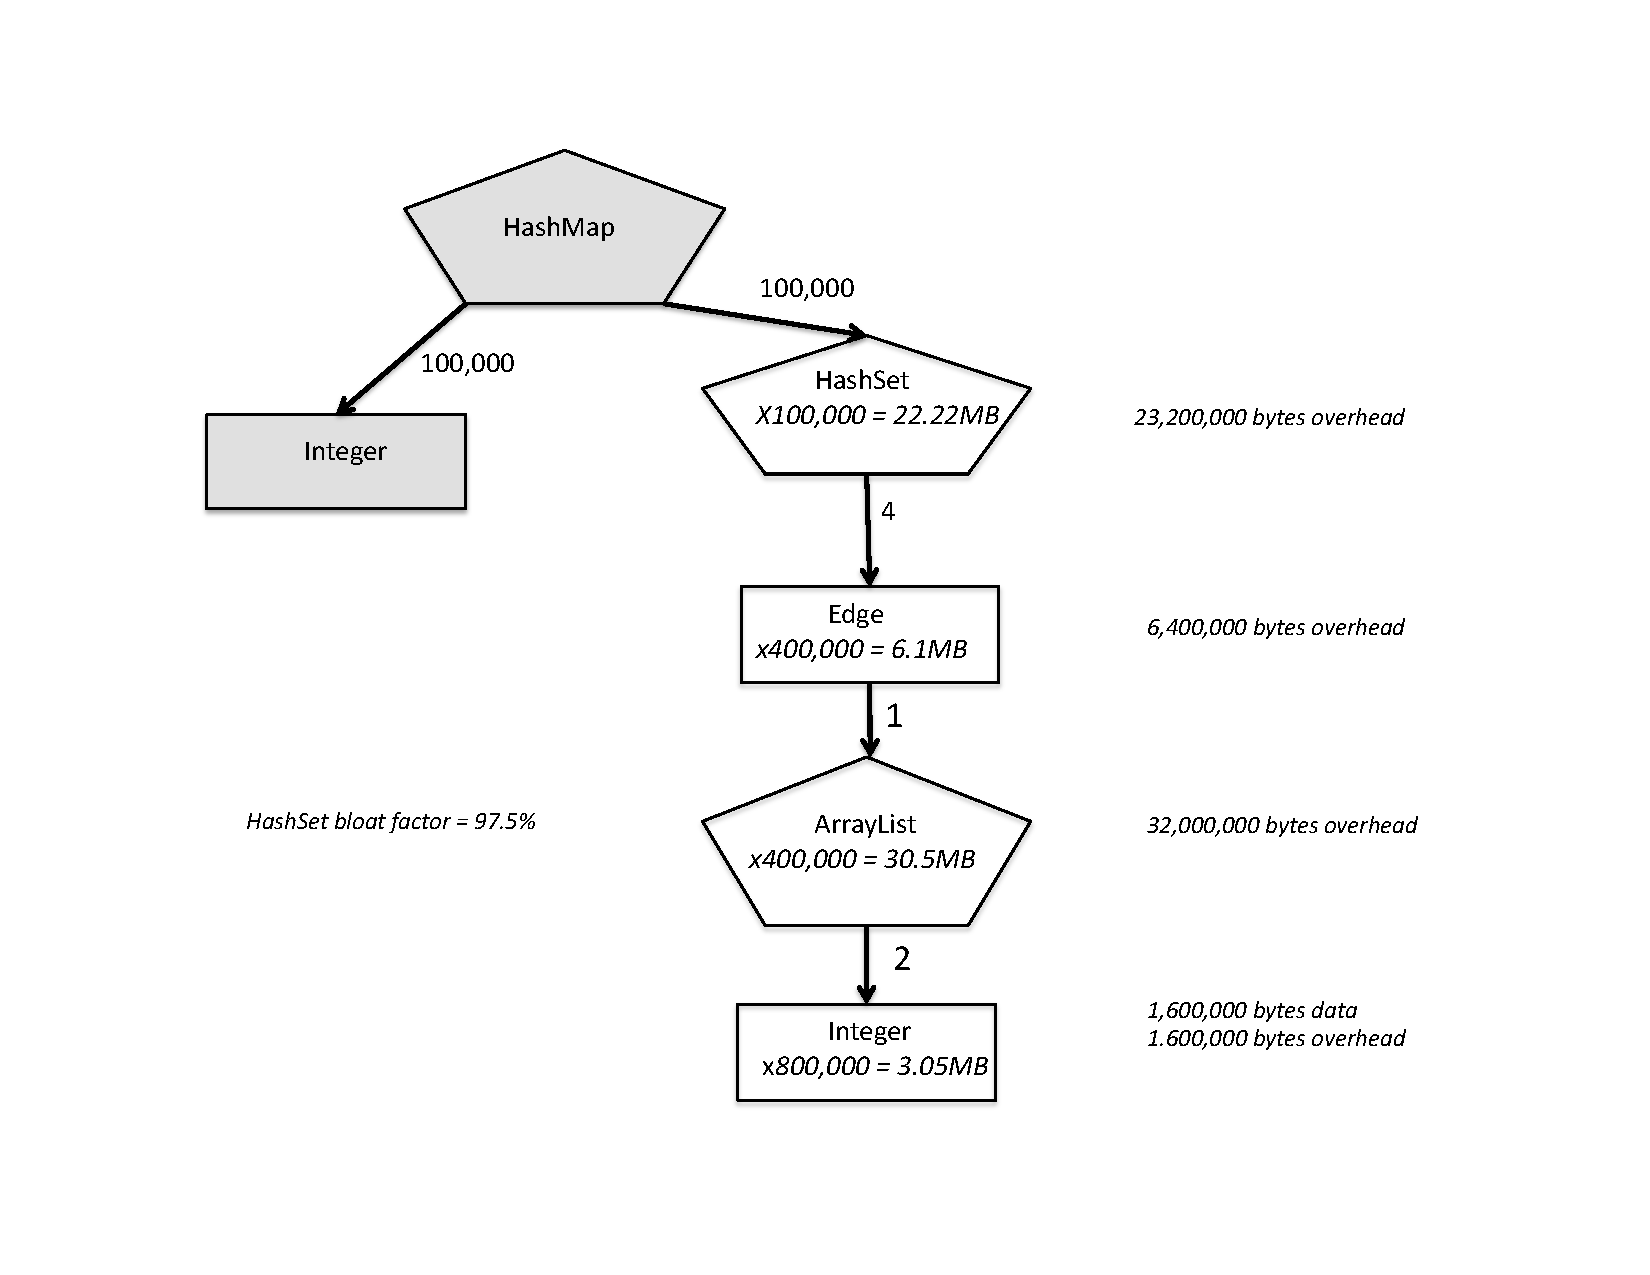
\includegraphics[width=.80\textwidth]{part3/Figures/graph-hashset.pdf}
  \caption{A 100,000-node graph, stored as a
  \class{HashMap} from nodes to \class{HashSets} of edges.}
  \label{fig:graph-hashset}
\end{figure}
%Sun library --  Empty HashSet -- 136 bytes
% 16 bytes HashSet (header + pointer)
% 40 byptes HashMap Object 
% 80 bytes empty array of entries

%HashMapEntry:  24 bytes:  header + 4 fields (value, key, next, hash)
% 4 entries -- 96 bytes
% total overhead for 4 entry hashset: 232 bytes
% 100,000 hashsets with 4 entries is 22.125MB

% HashMap size: 40 for header + 8 for array header
% 24 bytes per entry + 6 per entry in the array (assume extra for growth space)
% so for 100,000 entries, thats 48 + 3,000,000 bytes = 2.86MB
%
% Edge 16*400,000 = 6.4 million = 6.1MB
%
% ArrayList container is 24 bytes (header, size, modcount, pointer) 
% Default array size os 10 -- 10*4+12 = 52 rounds to 56
% ArrayList is 80 (56+24) for 4 entries.
% 400,000 ArrayLists is: 32,000,000 bytes

This is a hugely bloated structure with a bloat factor of 95.7\%.
There are several problems here, that we will address one by one.
 The first problem is that edges are represented by 100,000 very small
 \class{HashSets}, each consuming 232 bytes, which is all overhead. It's hard to
 think of a good reason why such a heavy-weight collection should ever be used
 for storing just a few entries, and yet, this pattern arises in almost all
 applications. For small sets, \class{ArrayList} is almost always a better choice. 
 \class{HashSet} maintains uniqueness
  and provides fast access, but enforcing uniqueness
is not always needed. If uniqueness is
important, it can be enforced for an \class{ArrayList} 
 with a little extra checking code, and usually without significant performance
 loss when sets are small. Figure~\ref{fig:graph-arraylist} shows improved memory usage with
\class{ArrayList}. Each \class{ArrayList} incurs 80 bytes of overhead,
approximately a third the size of a \class{HashSet}.
 \begin{figure}
  \centering
 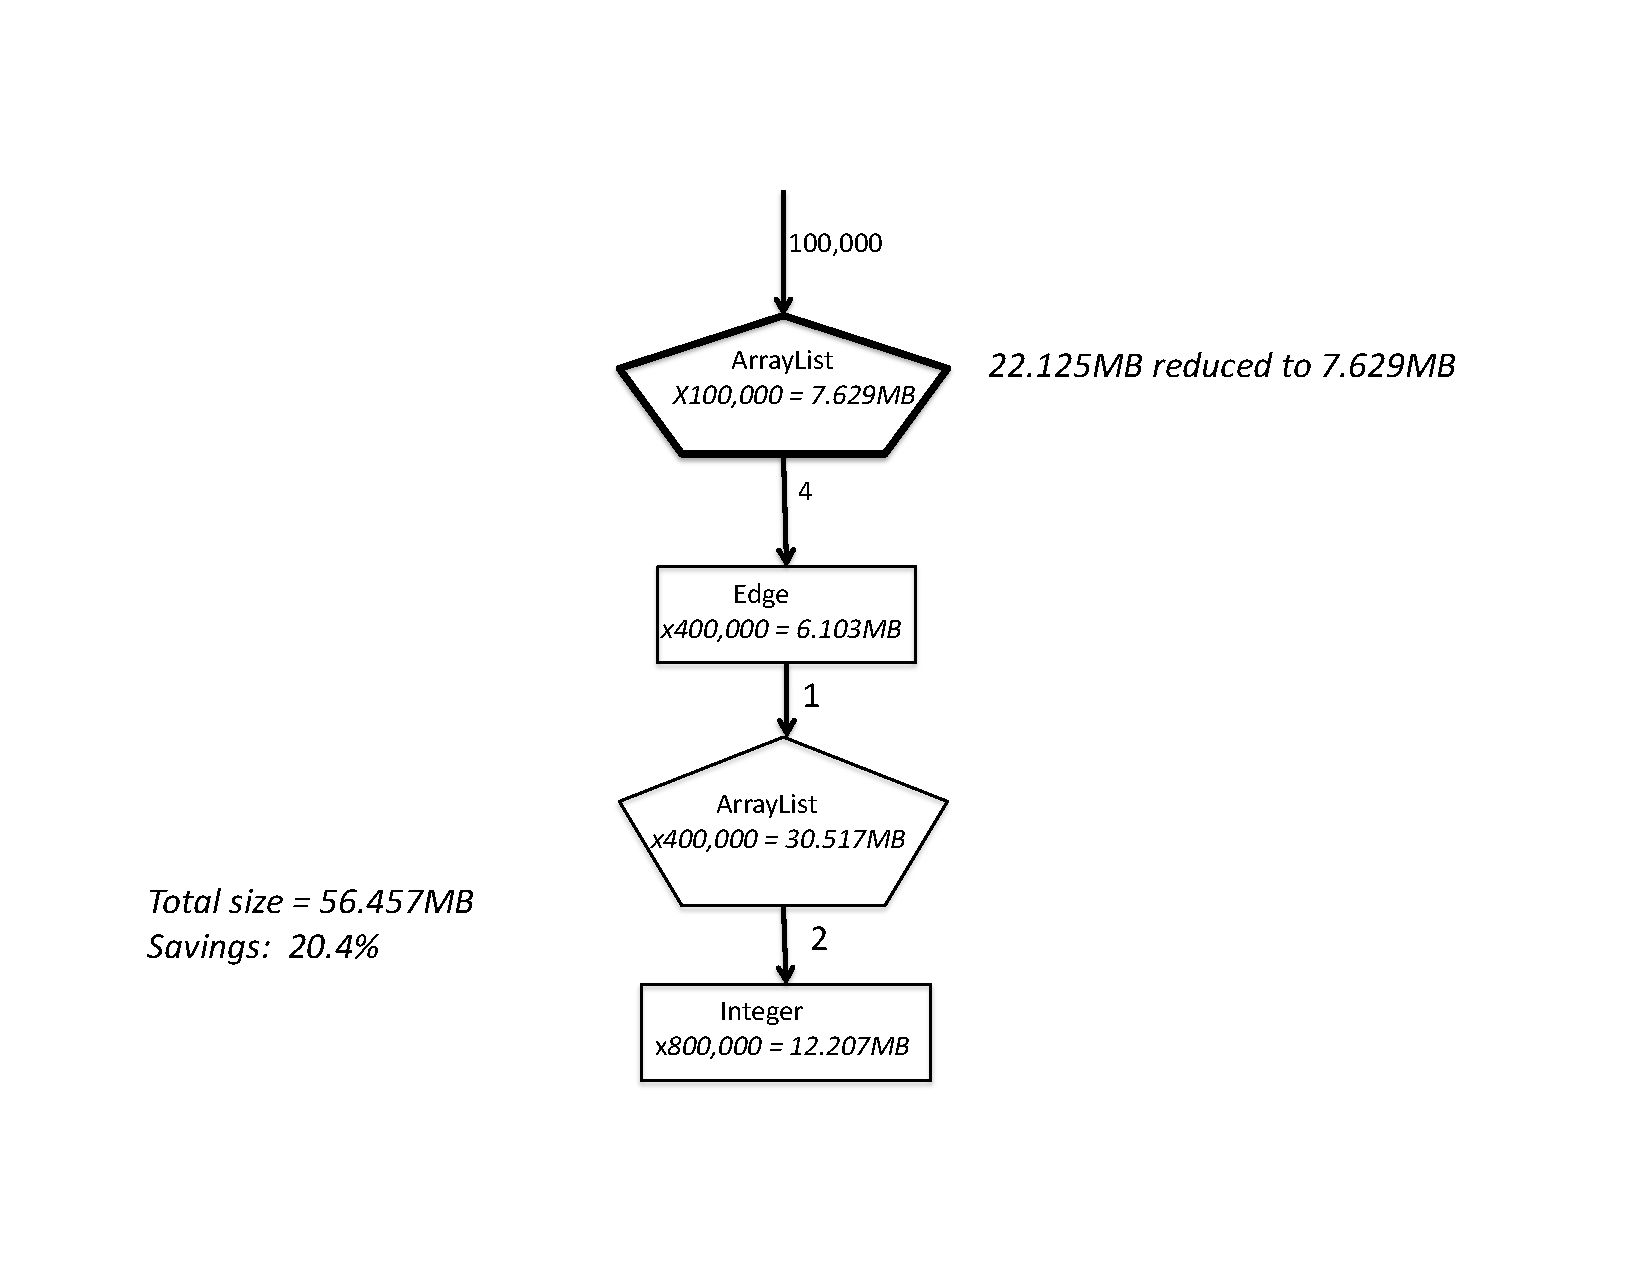
\includegraphics[width=.80\textwidth]{part3/Figures/graph-arraylist.pdf}
  \caption{A 100,000-node graph, stored as a
  \class{HashMap} from nodes to \class{ArrayLists} of edges.}
  \label{fig:graph-arraylist}
\end{figure}
This simple change saves 14.49MB, which is 20.4\%, but the bloat factor of
94.6\% is still quite large. This means that there is a lot of room for further
improvement, as we show later.

\section{The Cost Of Collections}
\label{sec:collectioncost}
Let's look at why a \class{HashSet} is so much bigger than an \class{ArrayList}. 
Some of the \class{HashSet} overhead is Java-related and
unavoidable. Other overhead is the result of hard-coded assumptions, for
example, the \class{HashSet} implementation assumes \class{HashSets} will be very large, 
and sacrifices memory space in favor of performance. 
Here is a breakdown of \class{HashSet} design decisions leading to
unnecessary bloat, as illustrated in Figure~\ref{fig:hashset}.
 \begin{figure}
  \centering
 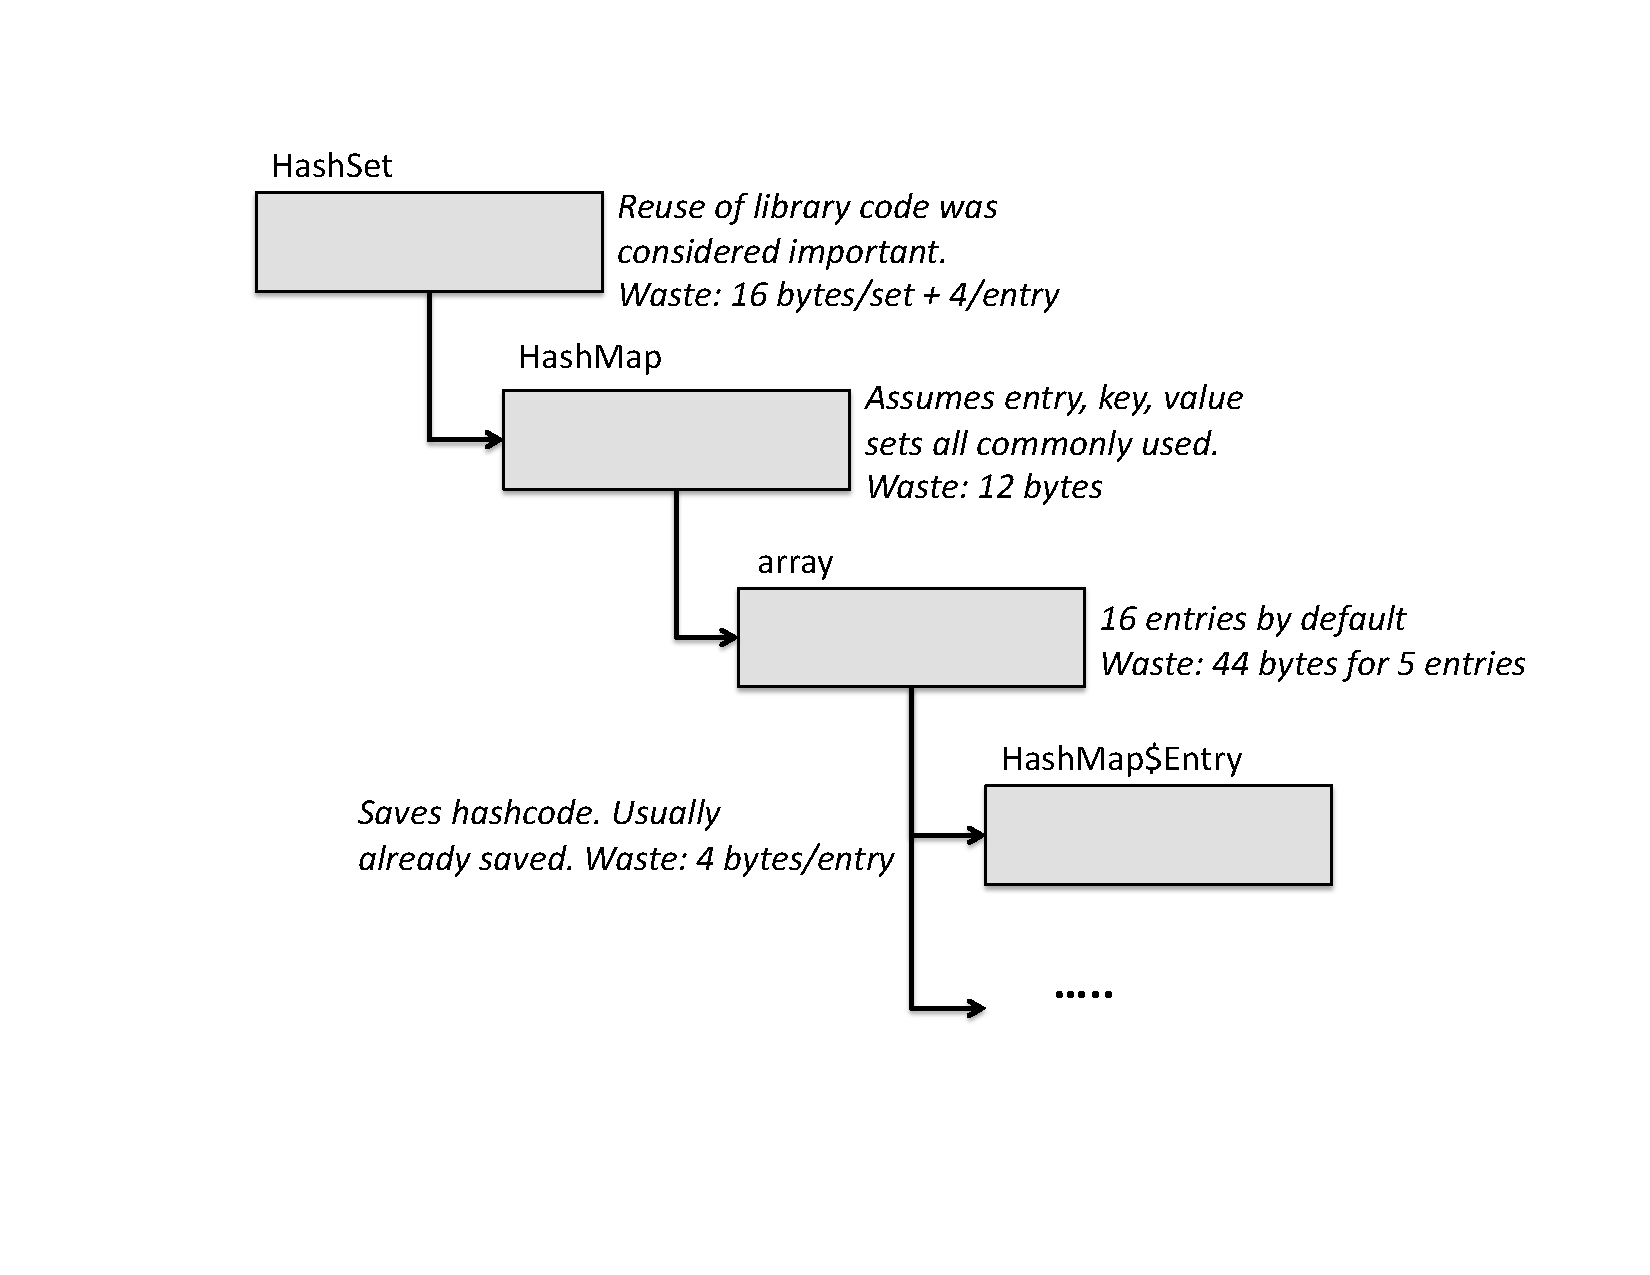
\includegraphics[width=.80\textwidth]{part3/Figures/hashset.pdf}
  \caption{The internal structure of a \class{HashSet} showing how
  implementation assumptions waste memory.}
  \label{fig:hashset}
\end{figure}

\paragraph{Reusing HashMap.} Internally, a \class{HashSet} is just a wrapper,
delegating all of its work to a \class{HashMap}.
This decision to reuse the \class{HashMap} code instead of specializing
\class{HashSet} costs an extra 16 bytes, which is reasonable if
\class{HashSets} are big and the fixed overhead costs are amortized away. 
Unfortunately, the fixed cost is multiplied when there are many
small \class{HashSets}. 
Also, \class{HashMap} is more general than what is needed for a \class{HashSet}.
Each \class{HashMap\$Entry} stores a key and a
value, and \class{HashSet} only uses the key, so four bytes are wasted per
entry. Sometimes specialization is a better option than reuse, especially for
library classes, where the usage patterns are not known in advance.
  
\paragraph{Open Chaining.} \class{HashMap} itself is fairly
 expensive. First, the \class{HashMap} object is just a container pointing
 to the actual array of entries. This delegation is necessary in Java.
 Secondly, \class{HashMap} uses an
 open chaining algorithm, which means that clashing entries are chained in a
 linked list. With open chaining, each entry requires its own
 \class{HashMap\$Entry} object and an extra level of indirection.
 
\paragraph{Default Array Size.} 
A \class{HashMap}, which is used to implement a \class{HashSet}, has a default
size of 16 entries, which means that its array of entries has an initial
size of 16. This wastes space when most \class{HashSets} have only a few
entries. For example, a \class{HashSet} with five entries wastes 44 bytes.


\paragraph{Bookkeeping Fields.} \class{HashMap} allows callers to iterate over
its set of keys, set of values, and set of entries. These sets are cached once
they are created. Every \class{HashMap} has three pointers
to store these sets, which is an extra 12 bytes.
However, its not that common to use
any of these sets, and very rare to use more than one set at a time.
 Certainly when the \class{HashMap} is part of a \class{HashSet}, 
there is never a need for a set of values.
  
 \paragraph{Extra Per-Entry Costs.} Each \class{HashMap\$Entry} stores a
 hashcode, which is an unnecessary redundant field. The most common keys are either
 \class{Strings}, which store their own hashcode, or \class{Integers}, whose
 hashcodes are easy to compute. 
\paragraph{}
In contrast, \class{ArrayList} has a smaller fixed cost and a smaller
per-entry cost than \class{HashSet}. It is really just an expandable array,
consisting of a wrapper object and an array of entries, as shown in Figure~\ref{fig:arraylist}. 
Lower fixed cost means that an \class{ArrayList} with just a few
 elements is smaller than a \class{HashSet} with the same elements. Fixed costs
 include wrapper objects and unitialized array elements. The fact that \class{HashSet}
 delegates to \class{HashMap} dramatically inflates its fixed cost. 
 \begin{figure}
  \centering
 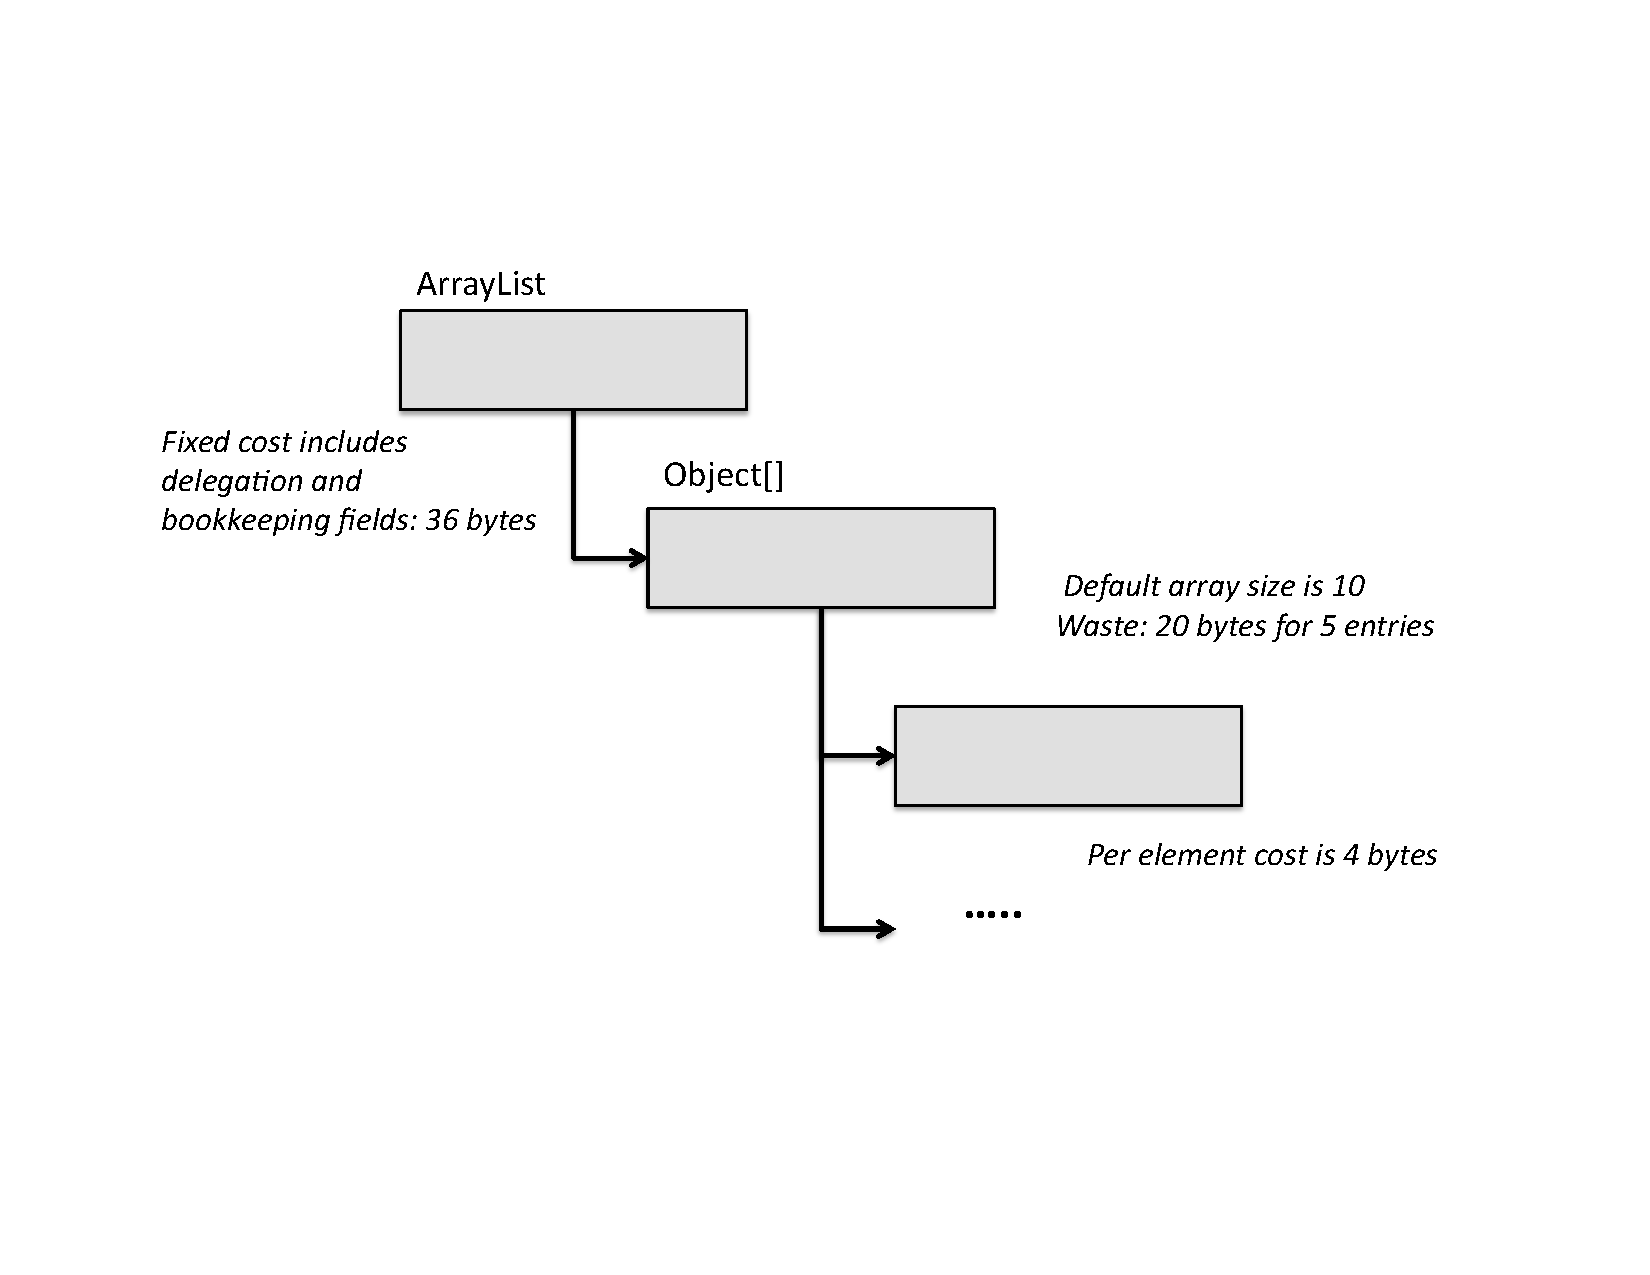
\includegraphics[width=.80\textwidth]{part3/Figures/arraylist.pdf}
  \caption{The internal structure of an \class{ArrayList}, which has a
  relatively low fixed overhead, and is scalable.}
  \label{fig:arraylist}
\end{figure}
 Lower per-entry cost means that
 \class{ArrayList} scales much better than \class{HashSet}. The per-entry cost
 of an \class{ArrayList} entry is an entry array pointer, which is 4 bytes.
 The per-entry cost of a \class{HashSet} is an entry array pointer plus a
 \class{HashMap\$Entry}, which is 28 bytes. So \class{ArrayList}  is better
 both for small and large sets.

Table~\ref{tab:collection-costs} shows the empty-collection costs of four basic
collections, \class{ArrayList}, \class{LinkedList}, \class{HashMap}, and \class{HashSet}. These costs have been
calculated based on the Sun JVM, using the techniques
described in Chapter~\ref{chapter:delegation}. The various other Java standard
library implementations in circulation have costs
similar to these. You can calculate them using the same methodology.

\begin{table}
  \centering
 %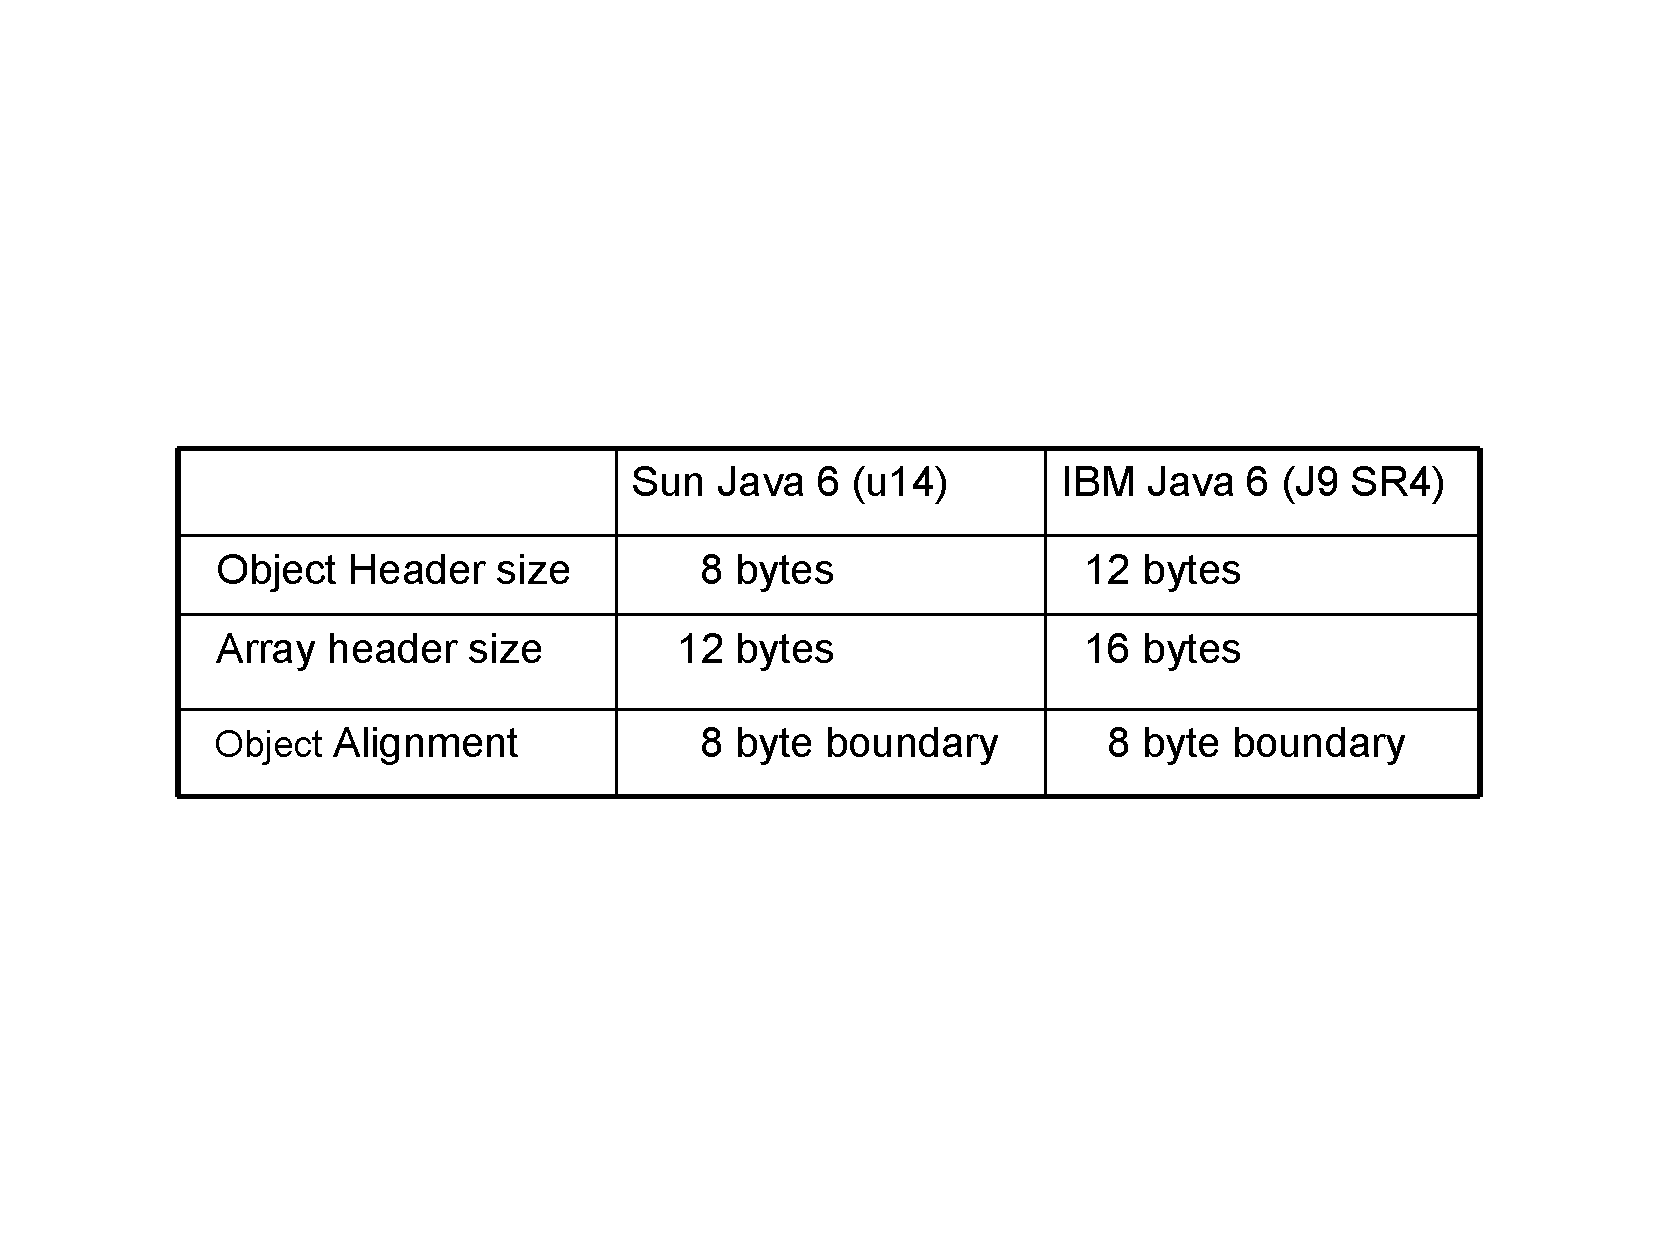
\includegraphics[width=.70\textwidth]{part2/Figures/chapter4/object-overhead.pdf}
 % 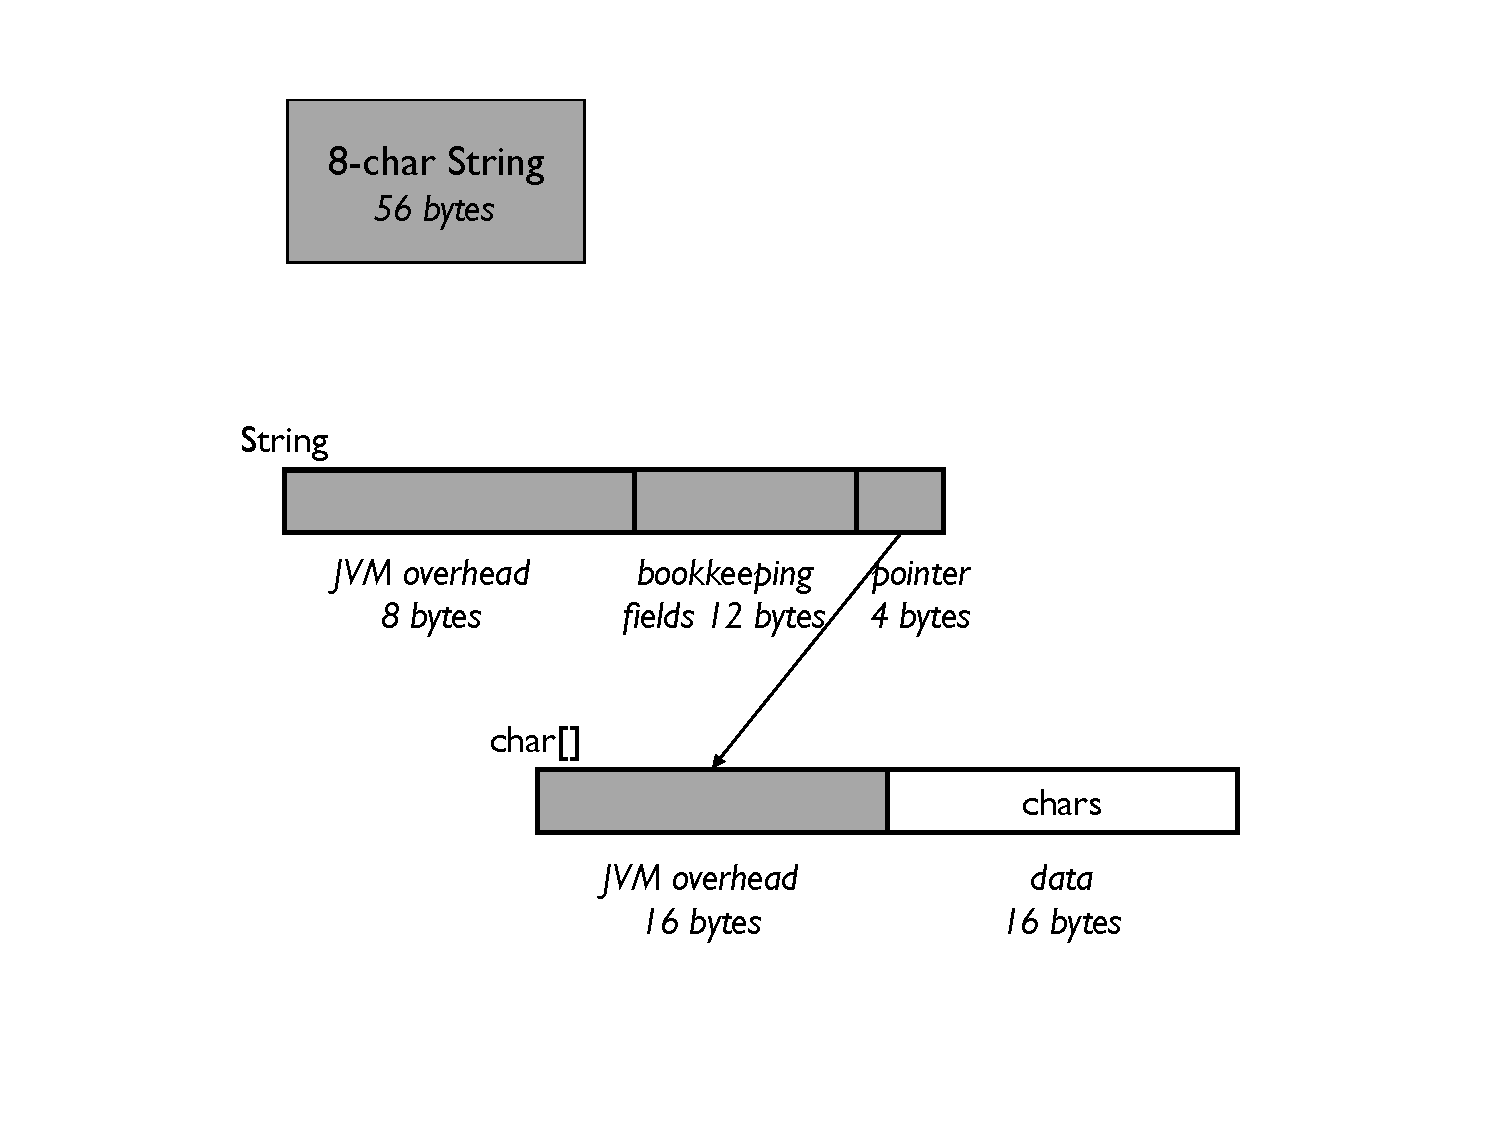
\includegraphics{eight-char-string}
 \begin{tabular}{llll} \toprule
 	 Collection & Fixed Cost & Per-Entry Cost & Default Capacity \\ \midrule
 	ArrayList & 80 bytes & 4 bytes & 10 entries \\
 	LinkedList & 48 bytes & 24 bytes & 1 sentinel entry \\
 	HashMap & 120 bytes & 28 bytes & 16 entries \\
 	HashSet & 136 bytes & 28 bytes & 16 entries \\
 	\bottomrule
 \end{tabular}
  \caption{The cost breakdown of four basic Java standard library collections
  with default size and no entries. The fixed cost includes an array whose
   size equals the default capacity. The per-entry cost is used to
  determine scalability.}
  \label{tab:collection-costs}
\end{table} 

\section{Properly Sizing Collections}

Collections such as \class{HashMap} and \class{ArrayList} store their entries in
arrays. When these arrays become full, a larger array is allocated
and the entries are copied into the new array.  Since allocation and copying
can be expensive, these entry arrays are always allocated with some extra
capacity, to avoid paying these growth costs too often. 
This is why the initial capacity of an \class{ArrayList} is 10 rather than zero
 or one, and why its capacity increases by
50\% when it is reallocated. 
Similarly, the capacity of a \class{HashMap} starts at 16, and grows by a
factor of 2 when the \class{HashMap} becomes 75\% full. 

These default policies trade space
for time, on the assumption that collections grow. However,
typical applications have hundreds of thousands of small collections that
don't grow. As a result, there is no performance gain, and the extra
empty array slots can add up to significant bloat problem. Unless you take explicit
action, element arrays are almost always too big.

 
 Fortunately, for \class{ArrayLists}, it is possible to right-size them. If you
 know that an \class{ArrayList} has a maximum size $x$ less than the default
 size, then it's worth passing $x$ as a parameter to the constructor. This sets the initial capacity of the
 \class{ArrayList} to $x$. However, if you are wrong and the \class{ArrayList}
 grows bigger than $x$, then it will grow by 50\%, which may
 be worse than just taking the default initial size.
 
 Alternatively, you can call the \code{trimToSize} method which shrinks the
 entry array by eliminating the extra growth space. Trimming reallocates and
 copies the array, so it is expensive to keep calling \code{trimToSize} while an
 \class{ArrayList} is still growing. Trimming is appropriate after
 it has been fully constructed and will never grow again. In fact, applications
 often have a build phase followed by a used phase. 
 \class{ArrayLists} can be trimmed
  between these two phases, so that the cost of reallocation and copying is
  paid only once.
 
 Returning to the graph example, all
 \class{ArrayLists} in Figure~\ref{fig:graph-arraylist} have the default
 capacity. If we assume that the the graph is built in one phase, and used in
 another phase, then it is possible to trim all of the \class{ArrayLists}.
 This should save quite a bit of space, since there are 100,000
 \class{ArrayLists} with four entries on average, and 400,000
 \class{ArrayLists} with two entries each. In fact, trimming these
 \class{ArrayLists} saves 15.2 million bytes, as shown in Figure~\ref{fig:trimmed-graph}. The
 total size is reduced by 32\%, and the bloat factor went from 96.7\% to
 95.3\%. This is still rather high, but there are more optimizations ahead.
 % 100,000 4 entry arrays == a 4 entry array is 32 bytes (16+12=28, rounds up
 % to 32)
 % So each array saves (56-32)=24 bytes.  100,000*24=2,400,000 bytes saved
 % = 1,600,000 bytes
 % 400,000 * (10-2)*4 = 12,800,000 byptes/ saves 32 bytes per arraylist
 % 32*400000=12,800,000 saved   32,000,000 - 12,800,000 = 19,200,000

 \begin{figure}
  \centering
 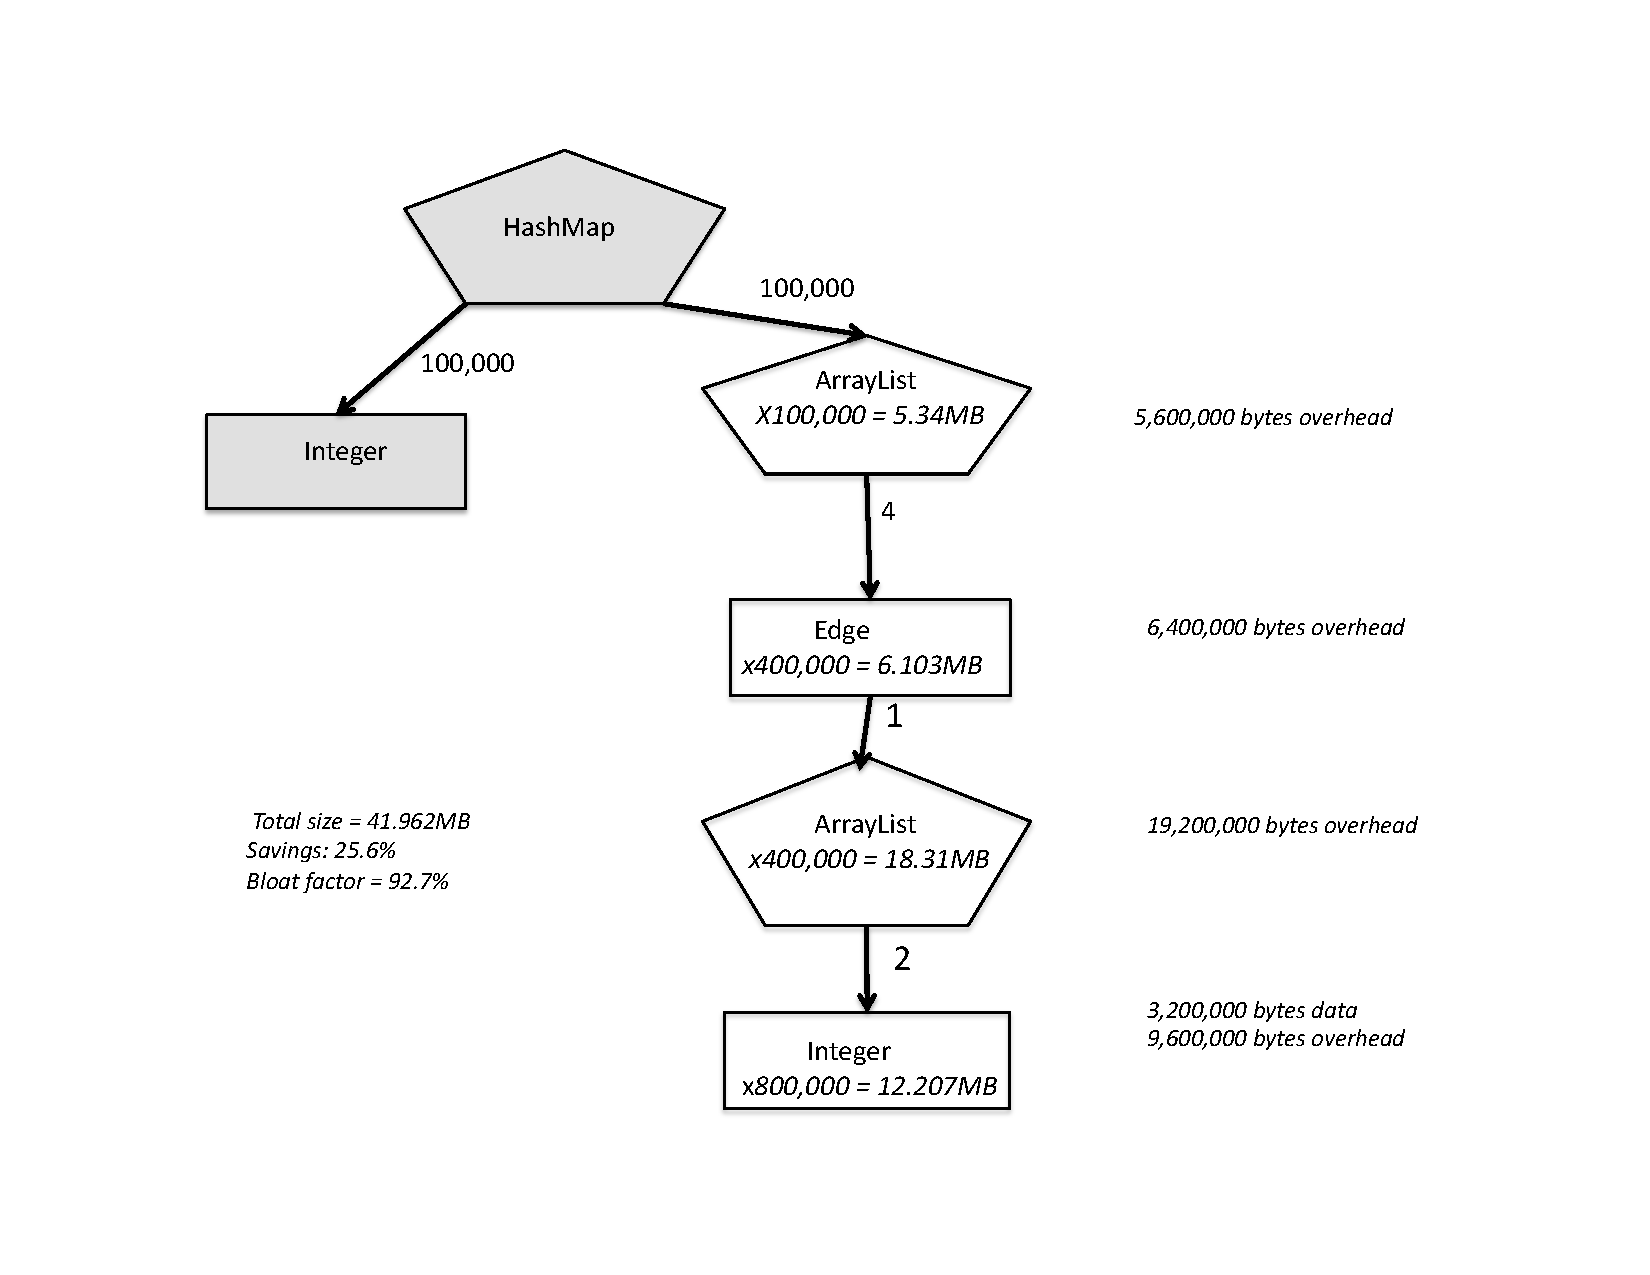
\includegraphics[width=.80\textwidth]{part3/Figures/trimmed-graph.pdf}
  \caption{The graph example after all of the \class{ArrayLists} have been
  trimmed by calling the \code{trimToSize} method.}
  \label{fig:trimmed-graph}
\end{figure}
 
\class{HashSets} and \class{HashMaps} do not have \code{trimToSize} methods.
but it is possible to pass the initial capacity and load factor as constructor
parameters when creating a \class{HashSet} or \class{HashMap}. 
However, before changing the initial capacity, you should
to ask yourself whether using a \class{HashSet} or \class{HashMap} at all is a
wise decision. If you are going to end up with many collections with fewer
than 16 elements, perhaps there is a more memory-efficient solution, like
\class{ArrayList}.
  
A \class{LinkedList} is another alternative for small collections, and are
better than \class{ArrayLists} if the collections are changing a lot. The
24 byte per-entry cost is larger, but there is no element array, and only one
extra entry, which is a sentinal.

\section{Avoiding Empty Collections}

Too many empty collections is another common problem. A quick look inside empty
collections shows that they are not all that empty. All the standard Java collections
eagerly allocate their subsidiary objects, which means that every empty
collection consists of two objects, including two object headers, a pointer,
plus whatever bookkeeping fields they have. 
According to Table~\ref{tab:collection-cost}, an empty \class{HashMap} consumes
120 bytes, and an empty \class{ArrayList} consumes 80
bytes, assuming a default initial size. 
Even if the initial size is zero, empty collections are still
large. A zero-sized \class{HashMap} consumes 56 bytes, and a zero-sized
\class{ArrayList} consumes 40 bytes. Empty \class{HashSets} are even bigger.

An empty collection problem is caused by eager initialization, that is,
allocating collections before they are actually needed, and often they are
never eventually needed. When an application allocates an empty
collection before it is needed, the collection class allocates an empty
array before it is needed, which is why there is so expensive. 

Suppose the graph
in Figure~\ref{fig:trimmed-graph} was initialized by the code:
\begin{shortlisting}
ArrayList nodes;
HashMap graph;
int numNodes;
   ..
   public void initGraph() {
       ..
       for (i = 0; i < numNodes; i++) {
          graph.put(nodes.get(i), new ArrayList());
       }
   }
\end{shortlisting}
Initially, each node is mapped to an empty edge \class{ArrayList}, so there are
100,000 empty \class{ArrayLists} before any edges are inserted. 
Suppose 25\% of the nodes in the final graph still have no
edges. Since edge \class{ArrayLists} have already been trimmed to size, 
each of the 25,000 empty \class{ArrayLists} consumes 40 bytes. If 
\class{ArrayLists} are allocated only for nodes with edges,
 .95MB can be saved, as shown in Figure~\ref{fig:empty-array}.
\begin{figure}
  \centering
 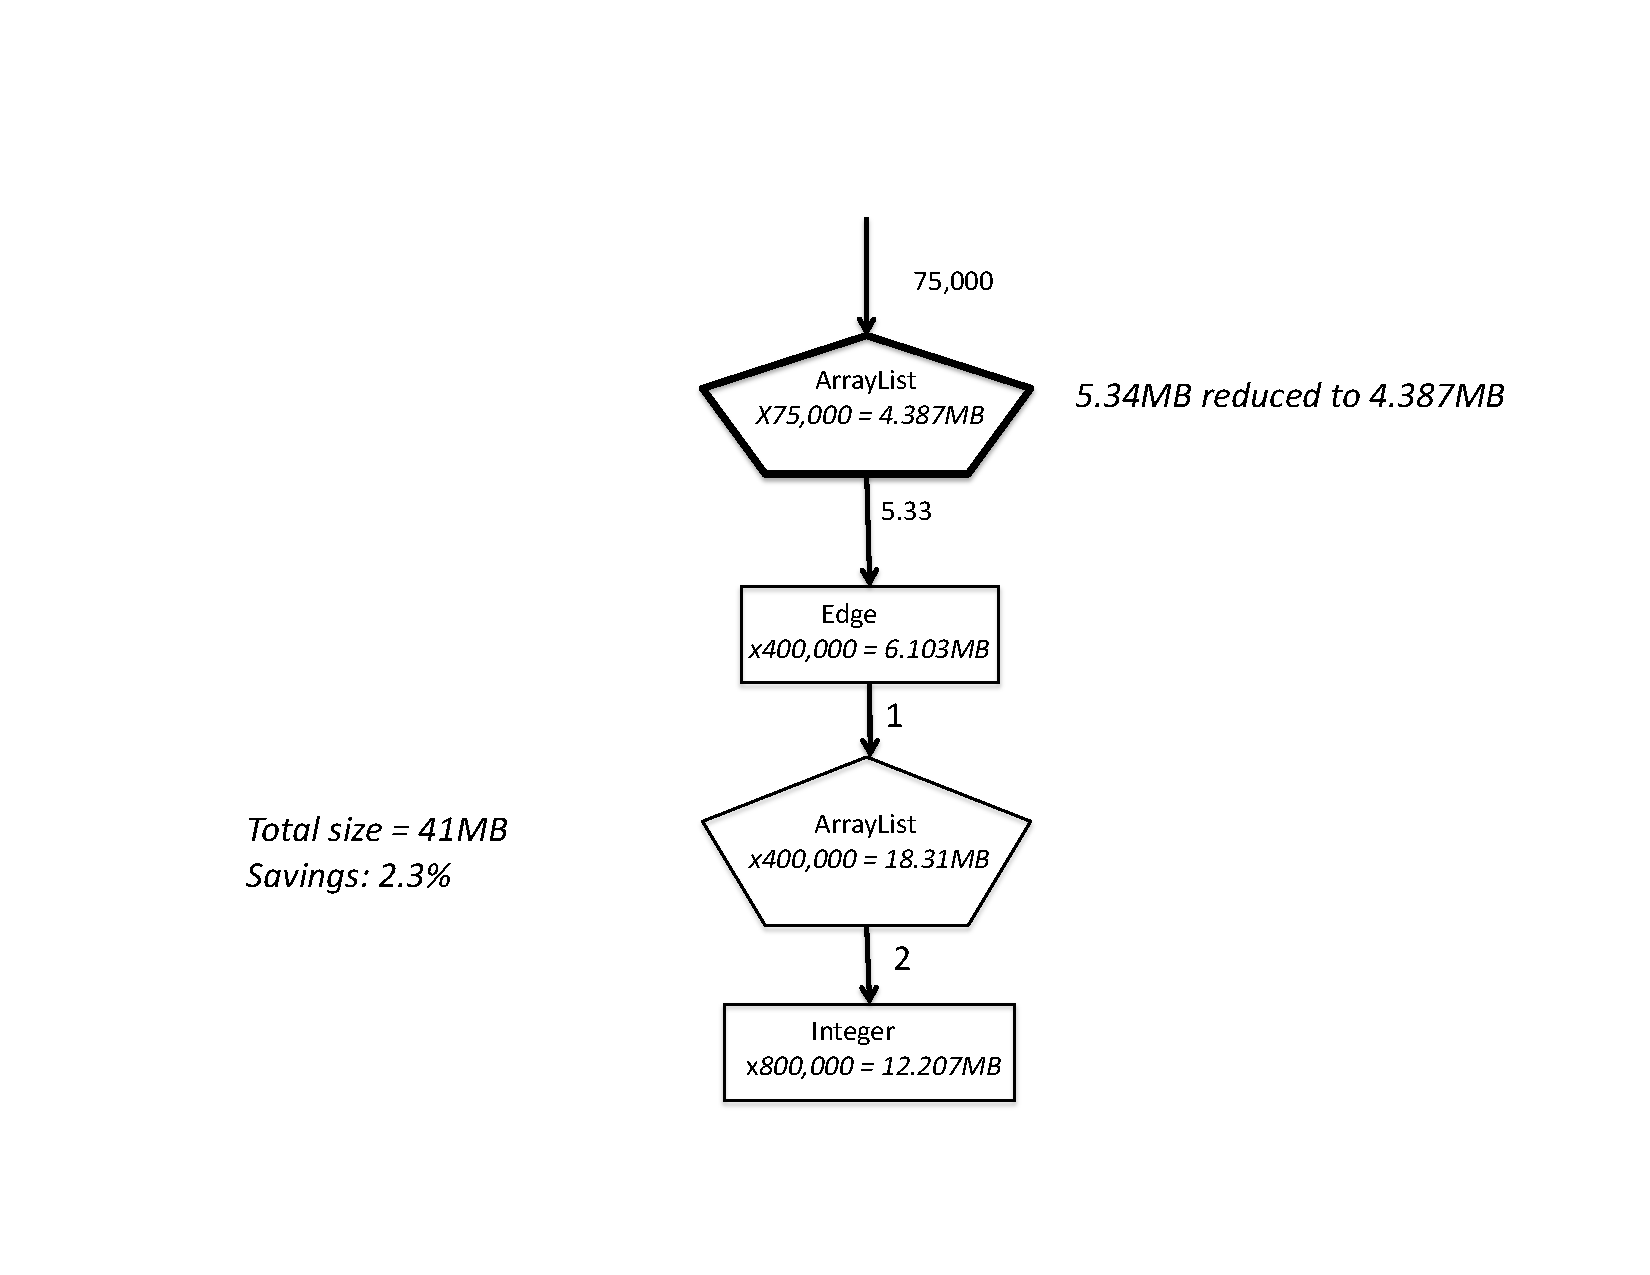
\includegraphics[width=.80\textwidth]{part3/Figures/empty-array.pdf}
  \caption{The graph example without initial empty \class{ArrayLists}.}
  \label{fig:empty-array}
\end{figure}
 
 In general, lazy allocation avoids creating too many empty collections.
 That is, instead of initializing all of the collections that you think you
 may need, allocate them on-demand, just before inserting an edge. On-demand
 allocation requires more checking code, to avoid \code{NullPointerExceptions}.
 
 Alternatively, you can initialize collection fields to reference static empty collections,
  including \code{EMPTY\_SET},
 \code{EMPTY\_LIST}, and \code{EMPTY\_MAP}. For example, 
 calling static method \code{Colletions.emptyList} to initialize edges 
 maps all nodes to a singleton immutable static \class{ArrayList}, and avoids
 creating empty \class{ArrayLists}:
 \begin{shortlisting}
 public void initGraph() {
       ..
       for (i = 0; i < numNodes; i++) {
          graph.put(nodes.get(i), Collections.emptyList());
       }
   }
 \end{shortlisting}
This code avoids checking whether the \class{ArrayList} exists at every use,
since for example, the size method and iterators work. However, you have to be
careful not to let the references to the static empty collections escape its
immediate context. 
If you give out any references to your collections before they�ve been
allocated, then there�s no way to update this escaped empty-collection reference
once an actual collection is allocated. 
 


\section{Fixed Size Collections}

Replacing \class{HashSet} by \class{ArrayList} helps, but it is not the end
of the story. The second problem in Figure~\ref{fig:graph-hashset} is the
implementation of \class{Edge}, which uses an \class{ArrayList} to store the
a target node and an edge label, both \class{Integers}. Even though
\class{ArrayList} is the least expensive collection, its functionality too
general to use for this purpose.
 

\section{Replacing Collections With Classes}
